\section{Sviluppi futuri}

Per quanto riguarda Random Forest, poiché l'algoritmo offre la possibilità di 
misurare l’importanza della variabile predittore, uno sviluppo futuro potrebbe 
essere utilizzare l'importanza delle variabili, mostrata nella figura 
\ref{fig:rf_importance}, per classificare l'utilità delle variabili, ed 
utilizzare solo le più importanti come features del modello. 

\begin{figure}[H]
	\centering
	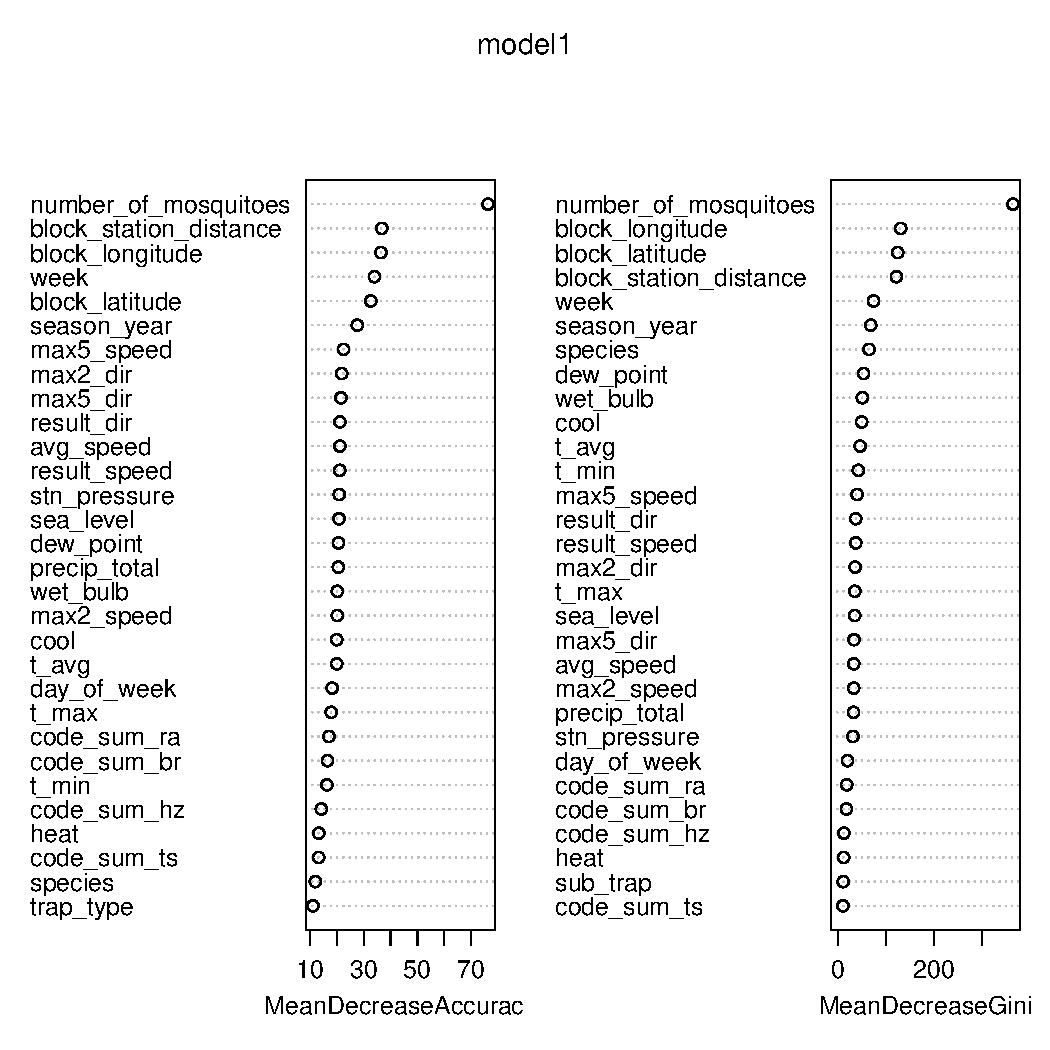
\includegraphics[width=0.7\columnwidth]{images/ml/random_forest/model_importance}
	\caption{Random Forest Importance}
	\label{fig:rf_importance}
\end{figure}

% FIXME: questa parte non la metterei ma per il momento la scrivo 
L'importanza variabile "globale" è la diminuzione media della precisione su 
tutte le previsioni out-of-bag con convalida incrociata. 
L'importanza variabile locale è la diminuzione media della precisione 
di ogni singola previsione out-of-bag con convalida incrociata. 

L'importanza di GINI misura il guadagno medio di purezza mediante la 
divisione di una determinata variabile. Se la variabile è utile, tende a 
dividere i nodi con etichetta mista in nodi di una singola classe pura. La 
divisione con variabili permutate non tende né a incrementare né a diminuire la 
purezza dei nodi. 
Permutando una variabile utile, si tende a dare una diminuzione relativamente 
grande del guadagno gini medio. L'importanza di GINI è strettamente correlata 
alla funzione di decisione locale, utilizzata dalla foresta casuale per 
selezionare la migliore suddivisione disponibile. Pertanto, non ci vuole molto 
tempo extra per calcolare. D'altra parte, il guadagno gini medio nelle 
divisioni locali, non è necessariamente ciò che è più utile misurare, al 
contrario del cambiamento delle prestazioni generali del modello. 
L'importanza di Gini è di importanza generale inferiore a (basata sulla 
permutazione) in quanto è relativamente più distorta, più instabile e tende a 
rispondere a una domanda più indiretta.
